\graphicspath{ {./img/intro/} }

\chapter{Introduction}

This set of lecture notes for the course {\bf Introduction to the Finite Element Method} is part of the learning resources used in the flipped class version of the subject adopted at Universidad EAFIT. In the flipped-class approach the students cover most of the theoretical aspects through independent home study, while the class time is invested in various learning activities conducted with support from the instructor and strongly based on peer-to-peer interaction. In this context, by collecting and summarizing fundamental numerical, theoretical and computational aspects required in the formulation of finite element algorithms, the lecture notes are intended to serve as a self-study guide . The notes are not as rigorous as material existing in published literature and are certainly not close in quality to excellent textbooks available in the subject. 

This introductory version of the course covers fundamental theoretical and computational aspects, required in the formulation of finite element methods as a numerical solution technique of boundary value problems. Although the studied algorithms are general the course evolves around the model of the linearized theory of elasticity. The fundamental theoretical framework is mainly covered in the lecture notes and in some referenced complementary material. The various theoretical topics are then associated to in-class learning activities involving some degree of computational work. Most of these activities are given in the form of Jupyter Notebooks.\footnote{Jupyter notebooks are open-source web applications used to create and share documents that contain live code, equations, visualizations and narrative text.}  In addition to the lecture notes and notebooks the authors have also developed {\bf SolidsPy}\footnote{https://github.com/AppliedMechanics-EAFIT/SolidsPy} a which is a complete Python-based finite element code to conduct stress analysis over arbitrary two-dimensional elastic domains. The code, which follows a modular structure facilitates the realization of learning activities in the form of (i) full stress analysis simulations (ii) implementation of intermediate steps aimed at covering the various steps in the FE algorithm and (iii) extensions to incorporate additional kinematical models. In the rest of this introductory chapter we present a simple problem of a mechanical spring-mass system which resembles the final form of a finite element algorithm and which serves to justify why we cover the material in the specific order proposed  here. Then we describe the topics covered in the notes and in the final part we indicate how to use the material.

\section*{Introductory problem}
\subsection*{A simple discrete system}
The simple case of a mechanical spring-mass system considered next resembles most of the algorithmic aspects of a finite element code. This system serves as a nice motivational example since the problem is already discrete thus avoiding the discussion of mathematical complexities. As will be presented throughout the course one of the goals of the finite element algorithm, when applied to a continuous system represented in terms of a boundary value problem, is to reformulate it as a discrete system fully analogous to the simple problem.

The system consists of an assemblage of masses joined by different springs submitted to time varying loads. For later purposes it is convenient to associate a spring with the concept of a finite element and a mass with a nodal point in a finite element algorithm.

The system may be like the one shown in \cref{fig:bathe} where the masses are represented by "cars" connected by springs (or finite elements) of different stiffness coefficients.

\begin{figure}[h]
\centering
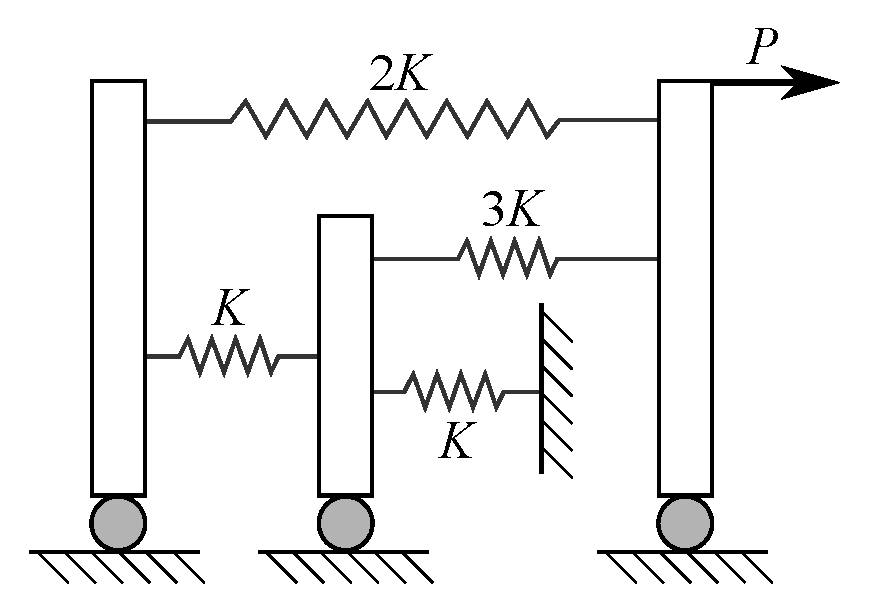
\includegraphics[width=8cm]{spring_system.pdf}
\caption{Typical assemblage of springs and masses.}
\label{fig:bathe}
\end{figure}


Considering a typical spring (or finite element), \cref{fig:springel}

\begin{figure}[h]
\centering
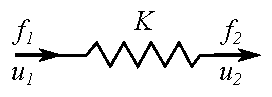
\includegraphics[width=6cm]{springel.pdf}
\caption{Typical spring element.}
\label{fig:springel}
\end{figure}

one finds that under a relative displacement $\delta u = u_1 - u_2$  the spring develops a force :

\[f_1 = K(u_1 - u_2)\]

while equilibrium of the spring requires

\[f_1 + f_2 = 0.\]

The force-displacement and equilibrium equations can be combined into:

\begin{equation}
    \begin{Bmatrix}
        f_1\\
        f_2
    \end{Bmatrix} =
    K\begin{bmatrix}
          1.0 & -1.0\\
        - 1.0 & 1.0
    \end{bmatrix}
    \begin{Bmatrix}
        u_1\\
        u_2
    \end{Bmatrix}.
    \label{eq:Kspring}
\end{equation}

\Cref{eq:Kspring} resembles a first fundamental aspect displacement based finite element methods which is the fact that the problem is described in terms of displacements of specific points (or nodes) and where internal element forces are found from these nodal displacements via a constitutive relationship. In the case of a continuous problem an analogous force-displacement relationship is established using interpolation theory together with equilibrium statements.


On the other hand, the equilibrium equation for a typical mass $m_j$ with displacement $u_j$  (see \cref{fig:dclmass}) and assumed to be attached to springs $i$ and $i+1$ reads
\begin{equation}
f_2^i + f_1^{i + 1} + m_j \dv{V_j}{t} = P_j.
\label{eq:equilmass}
\end{equation}

This equation can be written in terms of displacements after expressing the involved forces $f_2^i$ and $f_1^{i + 1}$ using terms from equations like \ref{eq:Kspring}

\[(K^i + K^{i + 1}) u_j - K^i u_{j - 1} - K^{i + 1} u_{j + 1} + m_j\dv{V_j}{t} = P_j .\]


\begin{figure}[H]
\centering
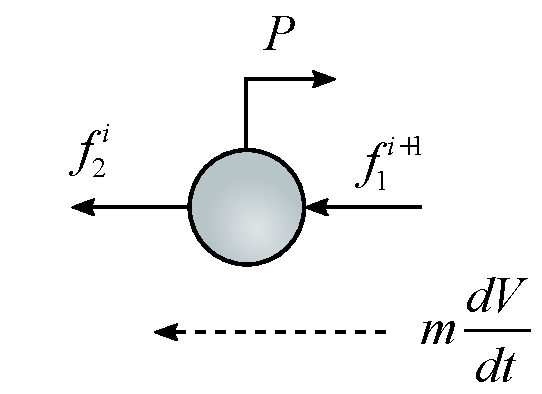
\includegraphics[width=6cm]{dcl_mass.pdf}
\caption{Free body diagram for a typical mass connected to springs $i$ and $i+1$.}
\label{fig:dclmass}
\end{figure}


Writing the elemental equilibrium equations for the springs in terms of the corresponding mass displacements $u_{j - 1}$, $u_j$ and $u_{j + 1}$ and generalizing the coefficients notation we get:

\[\left\{ {\begin{array}{*{20}{c}}
{f_1^i}\\
{f_2^i}
\end{array}} \right\} = \left[ {\begin{array}{*{20}{c}}
{k_{11}^i}&{k_{12}^i}\\
{k_{21}^i}&{k_{22}^i}
\end{array}} \right]\left\{ {\begin{array}{*{20}{c}}
{{u_{j - 1}}}\\
{{u_j}}
\end{array}} \right\}\]

and

\[\left\{ {\begin{array}{*{20}{c}}
{f_1^{i + 1}}\\
{f_2^{i + 1}}
\end{array}} \right\} = \left[ {\begin{array}{*{20}{c}}
{k_{11}^{i + 1}}&{k_{12}^{i + 1}}\\
{k_{21}^{i + 1}}&{k_{22}^{i + 1}}
\end{array}} \right]\left\{ {\begin{array}{*{20}{c}}
{{u_j}}\\
{{u_{j + 1}}}
\end{array}} \right\}\]

which gives for the equilibrium equation of the $m_j$ mass:

\[k_{21}^i{u_{j - 1}} + (k_{22}^i + k_{11}^{i + 1}){u_j} + k_{12}^{i + 1}{u_{j + 1}} + {m_j}\frac{{d{V_j}}}{{dt}} = {P_j}.\]

If one the other hand we also consider the contributions from the springs $K^i$ and $K^{i+1}$ to the equilibrium of masses $m_{j-1}$ and $m_{j+1}$ respectively we have the following matrix block:



\[\left[ {\begin{array}{*{20}{c}}
{}&{}&{}&{}\\
{}&{k_{11}^i}&{k_{12}^i}&{}\\
{}&{k_{21}^i}&{k_{22}^i + k_{11}^{i + 1}}&{k_{12}^{i + 1}}\\
{}&{}&{k_{21}^{i + 1}}&{k_{22}^{i + 1}}
\end{array}} \right].\]

Consideration of the complete system of masses leads to a system of linear equations of the general form


Considering now the complete system of masses and springs leads to a system of linear equations of the form
\begin{equation}
\left[ {{K_G}} \right]\left\{ {{U_G}} \right\} + \left[ M \right]\left\{ {{A_G}} \right\} = \left\{ {{F_G}} \right\}.
\label{eq:global}
\end{equation}
where each equation represents the equilibrium of a given mass.

The process of forming these global coefficient matrices by adding the contribution from different elements (springs) to the equilibrium equations of the different masses is known as element assembly and this can be achieved in a systematic way by establishing the connection between the global and local degrees of freedom. This can be accomplished through an operator storing in each row the global degrees of freedom corresponding to each element. For instance, \cref{fig:IBC} shows elements $K^i$ and $K^{i+1}$ and the global degrees of freedom corresponding to masses $m_{j-1}$, $m_j$ and $m_{j+1}$. The corresponding entries of the $DME$ operator for these elements are given by:


\[DME = \left[ {\begin{array}{*{20}{c}}
{}&{}\\
{j - 1}&j\\
j&{j + 1}\\
{}&{}
\end{array}} \right]\]

\begin{figure}[H]
\centering
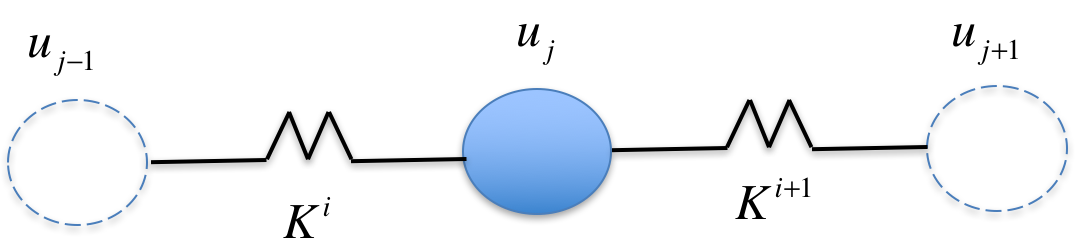
\includegraphics[width=12cm]{ibc}
\caption{Global degrees of freedom connected to the spring elements $K^i$ and $K^{i+1}$ respectively.}
\label{fig:IBC}
\end{figure}

and the assembly process from the contribution of these elements to the global coefficient matrix for elements $i$ and $i+1$ proceeds as:


\[\begin{array}{l}
{K_{j - 1,j - 1}} \leftarrow {K_{j - 1,j - 1}} + k_{11}^i\\
{K_{j - 1,j}} \leftarrow {K_{j - 1,j}} + k_{12}^i\\
{K_{j,j - 1}} \leftarrow {K_{j,j - 1}} + k_{21}^i\\
{K_{j,j}} \leftarrow {K_{j,j}} + k_{22}^i
\end{array}\]

and

\[\begin{array}{l}
{K_{j,j}} \leftarrow {K_{j,j}} + k_{11}^{i + 1}\\
{K_{j,j + 1}} \leftarrow {K_{j,j + 1}} + k_{12}^{i + 1}\\
{K_{j + 1,j}} \leftarrow {K_{j + 1,j}} + k_{21}^{i + 1}\\
{K_{j + 1,j + 1}} \leftarrow {K_{j + 1,j + 1}} + k_{22}^{i + 1}
\end{array}\]

The system given by \cref{eq:global} and assembled with the aid of the $DME$ operator can be solved for the global displacements $U_G$ and later use these displacements to compute the element forces.

This algorithmic strategy of assembling the contribution from all the elements to formulate the global equilibrium equations of the system is typical of finite element methods. However in the case of a BVP the continuous system must be converted first into a discrete system through different numerical and mathematical methods. A broad description of the method is described in \cref{algo:springs}.

\begin{algorithm}[H]
    \SetAlgoLined
    \KwData{Problem parameters; NUMNP, NUMEL, NMATP}
    \KwResult{Displacements and spring forces}
    Create $DM$E operator\;
    Assemble $K^G$, $F^G$\;
    \While{$j \leq 1, NUMEL$}{
        $K^G \leftarrow K^G+K^i$\\
        $F^G \leftarrow F^G+F^i$\\
    }
    Solve $[K^G]U=F^G$\\
    Find internal forces
    \caption{Springs Algorithm.}
    \label{algo:springs}    
\end{algorithm}

The full implementation of the mass-springs system is given in an accompanying notebook in the course REPO.
\newpage
\section*{Contents of the course}
The course is divided in three parts as follows:

\begin{itemize}
\item Part 1 covers classical numerical methods such as interpolation theory and numerical integration within the context of finite element methods. These methods are shown to be fundamental in the conversion of the continuous system into a discrete system analogous to the discussed mass-springs system. The numerical methods are studied from its theoretical and computational aspects and the suggested learning activities are described in notebooks 1 through 6.

\item Part 2 presents the boundary value problem corresponding to the model of the linearized theory of elasticity and in particular its description through formulations which are suitable for a solution in terms of finite elements algorithms. The boundary value problem is covered in notebook 7.

\item Part 3 concentrates on the formulation of the elasticity boundary value problem in a finite element algorithm. The algorithm and several related aspects are covered in notebooks 8 through 11, while notebook 12 contains a brief reference to the course finite element code SoildsPy.
\end{itemize}

The main set of accompanying notebooks also includes NB-0 which makes an introduction to the use of notebooks and a quick reference to data flow structures in Python. The set of lecture notes also include an appendix section presenting some more mathematical aspects of the method and additional tools that may result useful depending on the student's abilities.


\paragraph*{How to follow the course?\footnote{{\bf This set of lecture notes and additional course material has been developed as part of the sabatical period of the first author and with the collaboration of the second author Nicolas Guarin-Zapata. The development of the notebooks and design of the learning activities in these notebooks has been developed thanks to the advisory of Camilo Vieira.}}}

The course and its different resources have been created to be used in a flipped class environment or as a self study material. In the formal course, as thought in the graduate program at Universidad EAFIT, it is recommended to follow the proposed sequence of activities starting with the section covering numerical methods as described previously.This same sequence is also recommended for independent learners with no previous knowledge on fundamental numerical methods like interpolation theory and numerical integration. More advanced students, with previous backgrounds on mathematical analysis and numerical methods can test their actual abilities by developing the activities proposed on NB-4 and NB-6 and then moving directly into Chapter 4 discussing the boundary value problem.




